%%%%%%%%%%%%%%%%%%%%
%% 03-METHODOLOGY %%
%%%%%%%%%%%%%%%%%%%%
\clearpage\section{Methodology / project development}

In order to construct our framework we had to develop a set of tools. Basically we developed two commands and a minimal web application:
\begin{itemize}
	\item{LXCE: command constructed on top of LXD}
	\item{LXCE-admin: }
	\item{Web-admin} 
\end{itemize}
\DUDA{explicar cada uno más detallado?? / los nombres de las herramientas en mayus o minus}

This chapter will provide with the technical implementation of each tool and how they are constructed and organized. 

%%% LXCE %%%
\subsection{LXCE}
The first tool developed in this thesis is what we have called 'lxce'.

It is basically a command line tool coded in Typescript built on top of the 'lxc' command line tool with the idea of improving the management and set up of the containers.
[TODO: site chapter]
\TODO{Site chapter}

We could already work only with the "lxc" tool but the problem is that in order to have a properly set up container we would have to do the following steps, for every container:
\begin{itemize}
	\item{Create the container with linux image specified}
		\begin{minted}[bgcolor=background, style=tango]{console}
[host]# lxc launch ubuntu:20.04 container
		\end{minted}
	\item{Configure password}
		\begin{minted}[breaklines,bgcolor=background,style=tango]{console}
[host]# lxc exec container -- bash -c "echo ${user}:${password} | chpasswd"
		\end{minted}
	\item{Set up shared folders}
		\begin{minted}[breaklines,bgcolor=background,style=tango]{console}
[host]# lxc config device add containers myfolder disk source=/www/data path=/data
		\end{minted}
	\item{Set up proxies, selecting each time a non used host port}
		\begin{minted}[breaklines,bgcolor=background,style=tango]{console}
[host]# lxc config device add myproxy proxy listen=tcp:0.0.0.0:4000 connect=tcp:10.1.2.1:80
		\end{minted}
\end{itemize}

Then, if we would like to access the containers by ssh or vnc we would have to create also the corresponding configuration files.

Everything is managed individually, which is good for a basic set up, but for situations where we are working with +50 containers is unmanageable. 

So the idea of this command is to resolve such limitations with a command which could:
\begin{itemize}
	\item{Manage containers by configuration files, with a default configuration file}
	\item{Organize containers by "domains"}
	\item{Be able to reference containers by aliases}
	\item{Configure proxies and shared locations with a configuration file}
	\item{Generate SSH and VNC configuration files to be distributed}
\end{itemize}

The architecture is the following:
\begin{figure}[H]
	\label{fig:LXCE architecture}
	\centering
	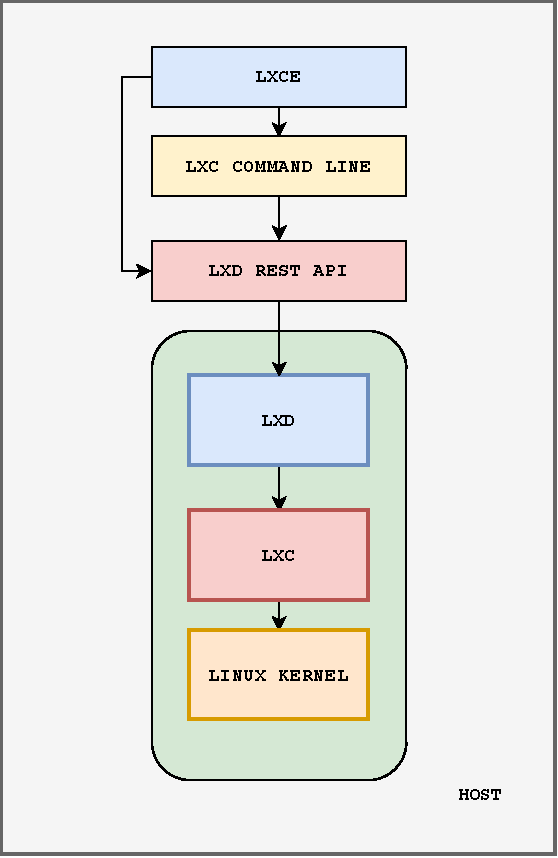
\includegraphics{img/03/lxce-diagram.pdf}
	\caption[LXCE block diagram]{\footnotesize{lxce architecture}}
\end{figure}

Once defined all the specifications for the command, we will explain how are the configuration files organized and the list of subcommands implemented.


\subsubsection{Configuration files}
Our command uses a series of configuration files for defining a list of properties (general and specific for each container). These configuration files are used by "lxce" and are updated acordingly.

The list of configuration files is the following:
\begin{itemize}
	\item{\textbf{container-default.conf}: default configuration file. Defines the default container configuration template}
	\item{\textbf{lxce.conf}: general command configuration. Defines properties such as the hostname of host}
	\item{\textbf{individual container configuration files}: they follow the container based template and are updated based on their properties}
	\item{\textbf{remmina}: defines a configuration file specific for a vnc client (remmina) }
	\item{\textbf{ssh}: ssh-config specific files for each container }
\end{itemize}

* see Appendix \ref{annex:lxce} for a further documentation of each subcommand
* see \cite{lxc}
\TODO{add the Remmina cite}

\subsubsection{Commands}
For the commands that are available for our command, we have develop the following commands:
\begin{itemize}
	\item{\textbf{lxce init}: initializes the command (configuration files and folder stucture)                         }
	\item{\textbf{lxce alias}: allow us to define custom names for the containers, as the container names are random}
	\item{\textbf{lxce delete}: deletes containers and configurations/folders related}
	\item{\textbf{lxce launch}: launch containers with folders/proxies/permissions configured acording to the configuration files                               }
	\item{\textbf{lxce list}: output a table of the current containers and their properties}
	\item{\textbf{lxce pass}: computes password of each container. They are all generated by a common seed that is stored in the main configuration file}
	\item{\textbf{lxce proxy}: configures the proxies associated to the containers }
	\item{\textbf{lxce rebase}: allow us to change a container base linux distribution without modyfying the container properties}
	\item{\textbf{lxce show}: outputs the container configuration files }
	\item{\textbf{lxce start}: start containers. Really conveninet to start a list of container from the same domain}
	\item{\textbf{lxce stop}: same as the start subcommand                                 }
	\item{\textbf{lxce uninstall}: removes all the configuration files and container running in the host }
\end{itemize}
* see ANNEX III for a complete description
\TODO{Add annex}

\newpage
%%% LXCE-ADMIN %%%
\subsection{LXCE-admin}
The second command implemented is intended to be used as an administration tool for managing the hosts with "lxce" installed.  

The idea is to have a central host with remote access to a list of hosts with the command line tool installed "lxce" in order to synchronize all configuration files from all the available hosts. 

Because with all the configurations files in a centralized location we have:
\begin{itemize}
	\item{Complete view of all the containers across different hosts}
	\item{Access to configuration files for SSH and VNC services}
	\item{Ability to compute password for remote access to containers}
\end{itemize}

The synchronization is done using a sync tool (rsync) that enable us to have synchronized folders between different hosts.

We can see how would look like in the following figure:
\begin{figure}[H]
	\label{fig:LXCE-ADMIN architecture}
	\centering
	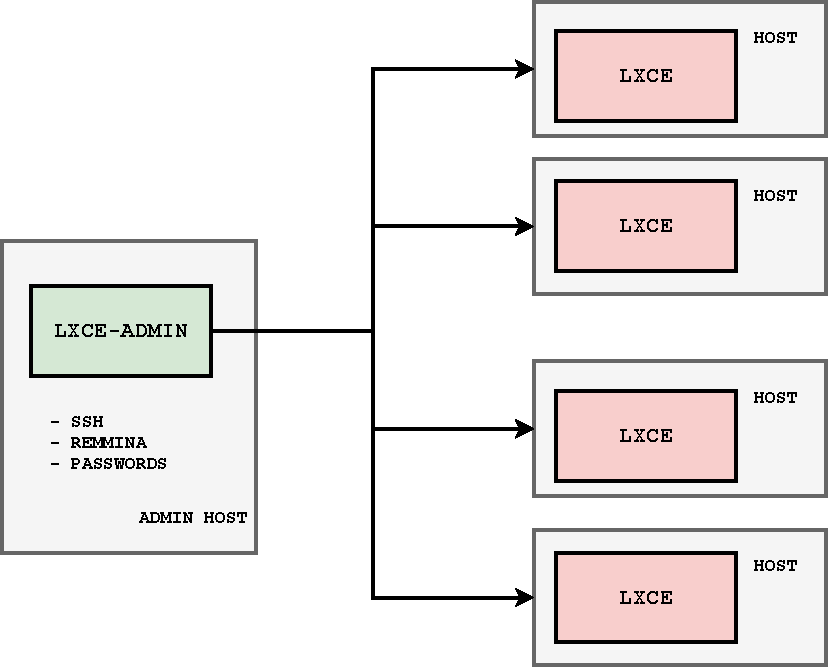
\includegraphics{img/03/lxce-admin-diagram.pdf}
	\caption[LXCE-ADMIN block diagram]{\footnotesize{lxce-admin architecture}}
\end{figure}


\subsubsection{Configuration files}
The files that must be syncronized are mainly:
\begin{itemize}
	\item{SSH: ssh-config files to be distributed and used by the admin host}
	\item{VNC: remmina configuration files to be used for the admin host and to be distributed}
\end{itemize}
in order to be able to use the command ssh correctly and have the automatic vnc configurations for the remmina VNC program (the command will also configure the passwords to be used along remmina).


\subsubsection{Commands}
The subcommands we have develop for the "lxce-admin" tool are:
\begin{itemize}
	\item{\textbf{lxce-admin config add}: configures a new host with lxce installed and syncronized all the configuration files for first time}
	\item{\textbf{lxce-admin config list}: list a table with the hosts configured and the total number of domains and containers}
	\item{\textbf{lxce-admin config remove}: removes a configured host and it's configuration files}
	\item{\textbf{lxce-admin config update}: syncronized configuration files from specific host}
	\item{\textbf{lxce-admin pass}: computes password for containers in specific host}
	\item{\textbf{lxce-admin remmina}: init remmona client into container}
	\item{\textbf{lxce-admin vnc}: starts a vnc connection with standar vnc client}
\end{itemize}
* see ANNEX III for a complete description

\newpage
%%% WEB-ADMIN %%%
\subsection{Web-admin}
The last tool implemented consist of a web application builded with React (framework of javascript) along with a minimal server providing a REST API in each host with "lxce" installed.

It is basically a web front-end for our framework that enables to view all our hosts and containers in a detailed view in real time.

\begin{figure}[H]
	\label{fig:Web admin architecture}
	\centering
	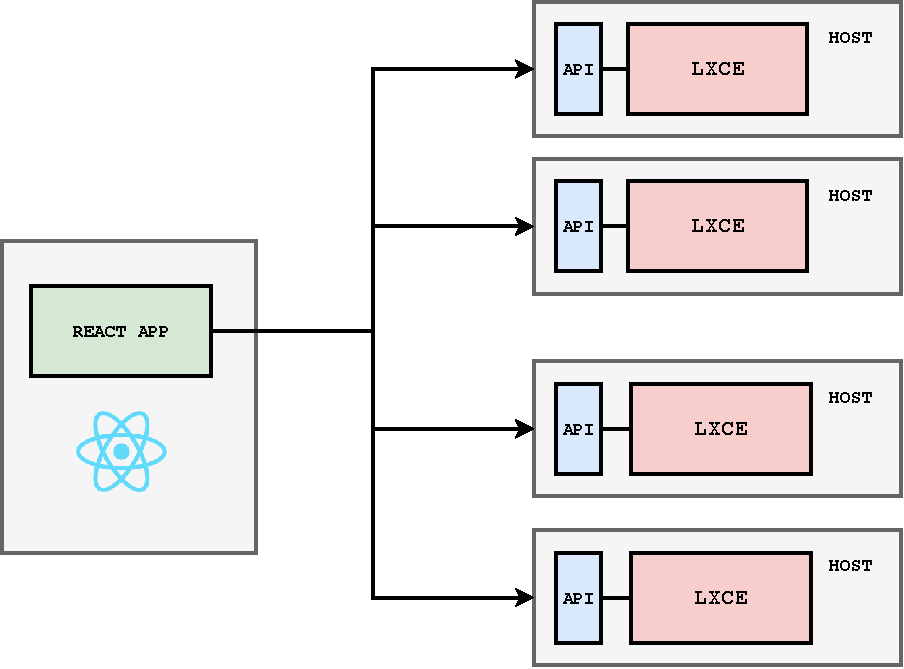
\includegraphics{img/03/web-admin-diagram.pdf}
	\caption[Web admin block diagram]{\footnotesize{web admin architecture}}
\end{figure}

It has only been implemented the view of the containers, but the idea of the web application is to be able to manage of all the "lxce" commands through the API provided and offer a web alternative for the "lxce-admin" command line tool.

For a detailed view of the API see ANNEX 
\TODO{put API ANNEX}


The API is provided by this simple express server:
\begin{minted}[bgcolor=background]{javascript}
const express = require("express")
const child = require("child_process")
const cors = require("cors")

const app = express()
const PORT = process.argv[2]

app.use(cors())

app.get("/containers", (req, res) => {
    const response = child.execSync("lxce list -f json").toString()

    res.setHeader('Content-Type', 'application/json');
    res.send(response)
})

app.listen(PORT, () => {
    console.log(`[*] Server listening on port ${PORT}`)
})
\end{minted}

\TODO{bibliography for React framework}
